\documentclass[12pt]{article}
\newcommand{\pdftitle}{periodic-boundary-conditions}
\input{preamble}


\newcommand{\ustar}{u^{\ast}}
\newcommand{\vstar}{v^{\ast}}

\pagestyle{fancy}
\fancyhead[L]{Periodic Boundary Conditions}
\fancyhead[C]{}
\fancyhead[R]{E. Torres}
\renewcommand{\headrulewidth}{1.0pt}
\fancyfoot[L]{\today}
\fancyfoot[C]{}
\fancyfoot[R]{\thepage}
\renewcommand{\footrulewidth}{1.0pt}

\begin{document}
\section{Finite difference schemes}
    \subsection{$u^{\ast}$ velocity}
The finite difference equations for the $\ustar$ velocity field are defined
below in Eqs.~(\ref{eq:star-left-boundary}-\ref{eq:star-right-boundary})
\begin{itemize}
    \item Left boundary (i.e., $i=\frac{1}{2}$ coding index \texttt{u(:,0)})
        \begin{subequations}
            \begin{equation}
                \begin{aligned}
                    u^{\ast}_{\frac{1}{2},j} = u^{n}_{\frac{1}{2},j} & -  \Delta t\Bigg[ 
                    \frac{
                        \big(u^{n}_{1,j}\big)^{2} - \big(u^{n}_{-1,j}\big)^{2}
                    }{\Delta x} +
                    \frac{
                        \left(uv\right)^{n}_{\frac{1}{2},j+\frac{1}{2}} - \left(uv\right)^{n}_{\frac{1}{2},j-\frac{1}{2}}
                    }{\Delta y}
                    \Bigg]\\
                    & + \Delta t \Bigg[
                        \frac{
                            u^{n}_{\frac{3}{2},j} - 2u^{n}_{\frac{1}{2},j} + u^{n}_{M+\frac{1}{2},j}
                        }{\Delta x^{2}}
                     + 
                        \frac{
                            u^{n}_{\frac{1}{2},j+1} - 2u^{n}_{\frac{1}{2},j} + u^{n}_{i+\frac{1}{2},j-1}
                        }{\Delta y^{2}}
                        \Bigg]
                \end{aligned}
            \end{equation}
            \text{where} 
            \begin{equation}
                u^{n}_{-1,j} = \frac{1}{2} \left(u^{n}_{\frac{1}{2},j} + u^{n}_{M+\frac{1}{2},j} \right)
            \end{equation}
            \label{eq:star-left-boundary}
        \end{subequations}
    \vspace{0.1in}
    \item Interior points (i.e., $i=\frac{3}{2}$ through $i=M-\frac{1}{2}$ coding index \texttt{u(:,1:M-1)})
        \begin{equation}
            \begin{aligned}
                u^{\ast}_{i+\frac{1}{2},j} = u^{n}&_{i+\frac{1}{2},j}  -  \Delta t\Bigg[ 
                \frac{
                    \big(u^{n}_{i+1,j}\big)^{2} - \big(u^{n}_{i-1,j}\big)^{2}
                }{\Delta x} +
                \frac{
                    \left(uv\right)^{n}_{i+\frac{1}{2},j+\frac{1}{2}} - \left(uv\right)^{n}_{i+\frac{1}{2},j-\frac{1}{2}}
                }{\Delta y}
                \Bigg]\\
                & + \Delta t \Bigg[
                    \frac{
                        u^{n}_{i+\frac{3}{2},j} - 2u^{n}_{i+\frac{1}{2},j} + u^{n}_{i-\frac{1}{2},j}
                    }{\Delta x^{2}}
                 + 
                    \frac{
                        u^{n}_{i+\frac{1}{2},j+1} - 2u^{n}_{i+\frac{1}{2},j} + u^{n}_{i+\frac{1}{2},j-1}
                    }{\Delta y^{2}}
                    \Bigg]
            \end{aligned}
        \end{equation}
    \vspace{0.1in}
    \item Right boundary (i.e., $i=M+\frac{1}{2}$ coding index \texttt{u(:,M)})
        \begin{subequations}
            \begin{equation}
                \begin{aligned}
                    u^{\ast}_{M+\frac{1}{2},j} = &u^{n}_{M+\frac{1}{2},j}  -  \Delta t\Bigg[ 
                    \frac{
                        \big(u^{n}_{M+1,j}\big)^{2} - \big(u^{n}_{M,j}\big)^{2}
                    }{\Delta x} +
                    \frac{
                        \left(uv\right)^{n}_{M+\frac{1}{2},j+\frac{1}{2}} - \left(uv\right)^{n}_{M+\frac{1}{2},j-\frac{1}{2}}
                    }{\Delta y}
                    \Bigg]\\
                    & + \Delta t \Bigg[
                        \frac{
                            u^{n}_{\frac{1}{2},j} - 2u^{n}_{M+\frac{1}{2},j} + u^{n}_{M-\frac{1}{2},j}
                        }{\Delta x^{2}}
                     + 
                        \frac{
                            u^{n}_{M+\frac{1}{2},j+1} - 2u^{n}_{M+\frac{1}{2},j} + u^{n}_{M+\frac{1}{2},j-1}
                        }{\Delta y^{2}}
                        \Bigg]
                \end{aligned}
            \end{equation}
            \text{where}
            \begin{equation}
                u^{n}_{M+1,j} = \frac{1}{2} \left(u^{n}_{M+\frac{1}{2}} + u^{n}_{\frac{1}{2}} \right)
            \end{equation}
            \label{eq:star-right-boundary}
        \end{subequations}
\end{itemize}

    \subsection{$v^{\ast}$ velocity}
The finite difference equations for the $\vstar$ velocity field, in the
periodic direction, are defined below in
Eqs.~(\ref{eq:v-star-left-boundary}-\ref{eq:v-star-interior-boundary}).
\begin{itemize}
    \item Left boundary (i.e., $i=0$ coding index \texttt{v(:,0)})
        \begin{subequations}
            \begin{equation}
                \begin{aligned}
                    v^{\ast}_{0,j+\frac{1}{2}} = v^{n}_{0,j+ \frac{1}{2}} & -  \Delta t\Bigg[ 
                    \frac{
                        \left(uv\right)^{n}_{\frac{1}{2},j+\frac{1}{2}} - \left(uv\right)^{n}_{-\frac{1}{2},j+\frac{1}{2}}
                    }{\Delta x} +
                    \frac{
                        \big(v^{n}_{0,j+\frac{1}{2}}\big)^{2} - \big(v^{n}_{0,j-\frac{1}{2}}\big)^{2}
                    }{\Delta y}
                    \Bigg]\\
                    & + \Delta t \Bigg[
                        \frac{
                            v^{n}_{1,j+\frac{1}{2}} - 2v^{n}_{0,j+\frac{1}{2}} + v^{n}_{M, j+\frac{1}{2}}
                        }{\Delta x^{2}}
                     + 
                        \frac{
                            v^{n}_{0,j+\frac{3}{2}} - 2v^{n}_{0,j+\frac{1}{2}} + v^{n}_{0,j-\frac{1}{2}}
                        }{\Delta y^{2}}
                        \Bigg]
                \end{aligned}
            \end{equation}
            \text{where} 
            \begin{equation}
                u^{n}_{-\frac{1}{2},j+\frac{1}{2}} = 
                                \frac{1}{2} \left(u^{n}_{M,j} + u^{n}_{M,j+1} \right)
            \end{equation}
            \begin{equation}
                v^{n}_{-\frac{1}{2}, j+\frac{1}{2}} =
                                \frac{1}{2} \left( v^{n}_{0, j+\frac{1}{2}} + v^{n}_{M, j+\frac{1}{2}} \right)
            \end{equation}

            \label{eq:v-star-left-boundary}
        \end{subequations}
    \vspace{0.1in}
    \item Interior points (i.e., $i=0$ coding index \texttt{v(:,1:M)})
        \begin{subequations}
            \begin{equation}
                \begin{aligned}
                    v^{\ast}_{i,j+\frac{1}{2}} = v^{n}_{i,j+ \frac{1}{2}} & -  \Delta t\Bigg[ 
                    \frac{
                        \left(uv\right)^{n}_{i+\frac{1}{2},j+\frac{1}{2}} - \left(uv\right)^{n}_{i-\frac{1}{2},j+\frac{1}{2}}
                    }{\Delta x} +
                    \frac{
                        \big(v^{n}_{i,j+\frac{1}{2}}\big)^{2} - \big(v^{n}_{i,j-\frac{1}{2}}\big)^{2}
                    }{\Delta y}
                    \Bigg]\\
                    & + \Delta t \Bigg[
                        \frac{
                            v^{n}_{i+1,j+\frac{1}{2}} - 2v^{n}_{i,j+\frac{1}{2}} + v^{n}_{i-1, j+\frac{1}{2}}
                        }{\Delta x^{2}}
                     + 
                        \frac{
                            v^{n}_{i,j+\frac{3}{2}} - 2v^{n}_{i,j+\frac{1}{2}} + v^{n}_{i,j-\frac{1}{2}}
                        }{\Delta y^{2}}
                        \Bigg]
                \end{aligned}
            \end{equation}
            \label{eq:v-star-interior-boundary}
        \end{subequations}
    \vspace{0.1in}
\item Right boundary (i.e., $i=M+1$ coding index \texttt{v(:,M+1)})\\

    Since $v$ is located at the cell center in the $i\text{-th}$ direction 
    the values at the right boundary can be simply copied from the 
    previously calculated left boundary.
        
\end{itemize}



    \newpage
    \subsection{Pressure}
The following finite difference equations were used to calculate the
pressure laplacian for the left boundary and interior points. 

\begin{itemize}
    \item Left boundary (i.e., $i=0$, coding index \texttt{p(:,0)})
        \begin{equation}
            p_{0,j} =   \frac{
                            p_{1,j} - 2p_{0,j} + p_{M,j}
                            }{\Delta x^{2}}
                            +
                        \frac{
                            p_{0,j+1} - 2p_{0,j} + p_{0,j}
                            }{\Delta y^{2}}
        \end{equation}
    \item Interior points (i.e., $i=1$ through $i=M$, coding index
        \texttt{p(:,1:M)})
        \begin{equation}
            p_{i,j} =   \frac{
                            p_{i+1,j} - 2p_{i,j} + p_{i-1,j}
                            }{\Delta x^{2}}
                            +
                        \frac{
                            p_{i,j+1} - 2p_{i,j} + p_{i,j}
                            }{\Delta y^{2}}
        \end{equation}
    \item Right boundary (i.e., $i=M+1$, coding index \texttt{p(:,M+1)}) \\
        \\
        Since the pressure is defined at the cell centers the pressure at 
        $i=M+1$ can be directly copied $i=0$, namely
        \texttt{p(:,M+1)=p(:,0)}.
\end{itemize}
            

    \begin{figure}[H]
        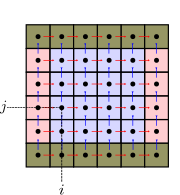
\includegraphics[height=0.5\textheight]{../../../media/periodic-BCs}
        \caption{Cell center periodic domain}
        \label{fig:periodic-domain}
    \end{figure}                                                            

\section{Testing results}
\subsection{Poiseuille's flow}
In order to test the periodic boundary conditions a one dimensional planar
Hagen-Poiseuille flow with an imposed pressure gradient was simulated and
compared to the analytical solution. The analytical solution is obtained
starting with the conservation of mass and momentum 
\begin{subequations}
    \begin{equation}
        \pdv{u}{x} + \pdv{v}{y} = 0
    \end{equation}
    \begin{equation}
        \pdv{u}{t} + \pdv{uu}{x} + \pdv{uv}{y} = 
                    - \pdv{p}{x} 
                    + \nu \left( \pdv{u}{x}{x} + \pdv{u}{y}{y} \right)  
        \label{eq:u-momentum}
    \end{equation}
    \begin{equation}
        \pdv{v}{t} + \pdv{uv}{x} + \pdv{vv}{y} = 
                    - \pdv{p}{y} 
                    + \nu \left( \pdv{v}{x}{x} + \pdv{v}{y}{y} \right)  
        \label{eq:v-momentum}
    \end{equation}
\end{subequations}

\begin{figure}[H]
    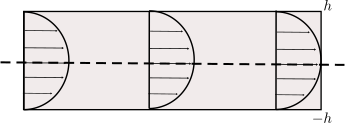
\includegraphics[width=0.5\textwidth]{../../../media/poiseuille-flow}
    \caption{Planar Hagen-Poiseuille flow}
\end{figure}

Where for steady one dimensional flow ($\mathbf{u} \equiv (u,v=0)$) 
the conservation of momentum reduces to    
\begin{equation}
    \nu \dv[2]{u}{y} = \dv{p}{x} = \text{const}
\end{equation}
Solving the above ODE and applying no slip boundary conditions at the
walls, $u(h)=u(-h)=0$, gives the exact analytical solution, namely 
\begin{subequations}
    \begin{equation}
        u(y) = u_{max} \left(1-\frac{y}{h^{2}}\right)
    \end{equation}
    \text{where}
    \begin{equation}
        u_{max} = -\dv{p}{x} \frac{h^2}{2\nu}
    \end{equation}
\end{subequations}

Figure~(\ref{fig:periodic-domain}) compares the cross sectional simulation
velocity profile to the exact Poiseuille flow solution.
\begin{figure}[H]
    \includegraphics[width=0.5\textwidth]{../data/data-64-dev/u-poiseuille.png}
    \caption{Cross sectional $u$ velocity}
    \label{fig:periodic-domain}
\end{figure}                                                            

\subsection{Taylor-Green Vortex}
In order to test the periodic boundary conditions on a more challenging
flow an additional simulation comparison was conducted on a unsteady
decaying Taylor-Green vortex problem. The Taylor-Green vortex is a
particular flow with the following specified initial conditions,   
\begin{subequations}
    \begin{equation}
        u(x,y,z,t=0)    = A \cos{ax} \sin{by} \sin{cz}
    \end{equation}
    \begin{equation}
        v(x,y,z,t=0)    = B \sin{ax} \cos{by} \sin{cz}
    \end{equation}
    \begin{equation}
        w(x,y,z,t=0)    = C \sin{ax} \sin{by} \cos{cz}
    \end{equation}
\end{subequations}
where it is easy to show from the continuity equation that $Aa + Bb +Cc =
0$. Therefore for a 2D simulation we can let $A=a=b=1$, $B=-1$, $c=\pi/2$,
and $C=0$. Thus giving the following exact solutions 
\begin{subequations}
    \begin{equation}
        u(x,y,t) =  \cos{x} \sin{y} F(t)
    \end{equation}
    \begin{equation}
        v(x,y,t) =  -\sin{x} \cos{y} F(t)
    \end{equation}
    \text{where}
    \begin{equation}
        F(t)    = \exp \left(-2 \nu t\right)
    \end{equation}
\end{subequations}
Figures~(\ref{fig:u-taylor-green} \& \ref{fig:v-taylor-green})
compare the $u$ and $v$ results to the exact Taylor-Green vortex solutions. 
\begin{figure}[H]
    \includegraphics[width=0.5\textwidth]{../../taylor-green-vortex/data/decay-data-2/u-velocity.png}
    \caption{$u$ velocity}
    \label{fig:u-taylor-green}
\end{figure}
\begin{figure}[H]
    \includegraphics[width=0.5\textwidth]{../../taylor-green-vortex/data/decay-data-2/v-velocity.png}
    \caption{$v$ velocity}
    \label{fig:v-taylor-green}
\end{figure}
\vfill


\end{document}
